\documentclass[11pt,a4paper]{report}
\usepackage[bahasa]{babel} %bahasa indonesia
\usepackage{graphicx} %gambar
\usepackage{sectsty}
\usepackage{setspace}
\usepackage{indentfirst}
\usepackage{url}

\renewcommand{\baselinestretch}{1.5} 
\chapterfont{\centering}

\author{Albert Kamord (2011730077)}
\title{3D Block-World-Problem-based Sudoku Games}
\begin{document}
\maketitle
\begin{abstract}

\indent Banyak pemain-pemain game zaman sekarang sudah tidak tertarik lagi dengan permainan tradisional. Dewasa ini, banyak orang yang lebih memilih permainan digital. Banyak permainan-permainan tradisional yang sudah dibuat versi digitalnya contohnya Sudoku. Walaupun sudah dibuat versi digitalnya, peminat permainan tradisional semakin menurun saja.

\indent Di dalam tulisan ini, akan disampaikan solusi untuk menarik kembali perhatian para \textit{gamers} dengan cara membuat simulator Sudoku di platform 3D. Simulator 3D ini akan dikaitkan dengan Block World Problem yang telah diketahui banyak orang. \\
\\
Kata kunci : \textbf{3D block world problem}
\end{abstract}

\tableofcontents \newpage 	% Daftar isi
\listoffigures \newpage 	% Daftar gambar


\chapter{Pendahuluan} %Pendahuluan
\section{Latar Belakang Masalah}
\indent Di zaman modern ini, banyak game digital yang sudah dibuat. Permainan-permainan sebelum era modern sudah dilupakan, contohnya Sudoku. Sudoku yang ada di zaman sekarang juga sudah dibuat versi digitalnya, tetapi peminat permainan ini semakin menurun saja. Sudoku pernah populer di seluruh dunia, terutama di kalangan orang-orang yang ingin mencoba kemampuan pikirannya.

\indent Perubahan zaman tentu saja menyebabkan banyak perubahan di dunia permainan juga. Dari permainan tradisional ke permainan yang menggunakan \textit{console}. Tentu saja permainan console juga mengalami perubahan. Awalnya, hanya permainan simple seperti tetris, kemudian permainan yang lebih kompleks seperti Super Mario Bros, sampai sekarang yang telah menggunakan teknologi-teknologi canggih untuk membuat sebuah game, contohnya Call of Duty.

\indent Banyak game digital yang telah dibuat dapat dibagi menjadi dua berdasarkan sudut pandang pemain, yaitu game 2D(dua dimensi) dan game 3D(tiga dimensi). Game 3D tentu saja lebih menarik perhatian daripada game 2D. Di dalam tulisan ini, akan disampaikan solusi untuk menarik perhatian pemain-pemain game dalam memainkan game Sudoku yang dikaitkan dengan Block World Problem dengan menggunakan Platform 3D.

\section{Rumusan Masalah}
Rumusan masalah yang terdapat di tulisan ini adalah:
\begin{enumerate}
	\item Mengapa jumlah peminat Sudoku semakin menurun?
	\item Apa solusi yang tepat untuk menaikkan jumlah peminat Sudoku?
\end{enumerate}

\section{Tujuan}
Tujuan dari tulisan ini adalah : Menarik perhatian gamers dengan menggunakan simulator Sudoku 3D yang dikaitkan dengan BWP dengan pandangan 3D. Tujuan lain adalah menyelesaikan suatu puzzle sudoku.

\chapter{Isi} %isi
\section{Sudoku}
\subsection{Definisi}
\indent Sudoku mulai populer sejak tahun 2004 di Inggris. Sudoku, atau Su Doku, berasal dari bahasa Jepang yang berarti Tempat Angka. Ide dari sudoku sangat simpel; pemain memiliki grid 9 x 9, dibagi menjadi 9 blok 3 x 3 :
\begin{figure}[h]
\centering
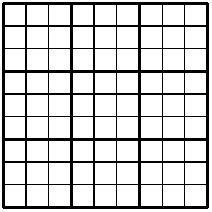
\includegraphics{sudoku}\\ \vspace{1cm}
\caption[Papan Permainan Sudoku]{Papan Permainan Sudoku} 
\end{figure}
Pada beberapa kotak tersebut, ada orang yang menempati atau menulis angka 1-9; tujuan dari pemain adalah untuk mengisi setiap kotak tersebut dengan catatan bahwa tiap baris, tiap kolom dan tiap blok 3 x 3 berisi hanya satu kali saja angka 1-9.
Pertanyaan yang sering ditanyakan adalah berapa banyaknya kemungkinan grid Sudoku. Artinya, berapa banyak cara yang dapat kita lakukan untuk mengisi kotak-kotak tersebut sesuai peraturan.

Dalam catatan ini, kami akan menjelaskan bagaimana kami pertama kali dihitung nomor ini. Ini adalah perhitungan pertama
nomor ini; kita harus menunjukkan bahwa ia telah kemudian dikonfirmasi menggunakan lainnya (lebih cepat!) metode.
Pertama, mari kita melihat bahwa grid Sudoku adalah kasus hanya khusus kotak Latin; ingat bahwa
Persegi latin order n adalah n × n persegi yang berisi masing-masing angka 1, ..., n di setiap baris dan kolom.
Perhitungan jumlah kotak Latin itu sendiri merupakan masalah yang sulit, dengan tidak ada rumus umum
dikenal. Jumlah kotak Latin ukuran hingga 11 × 11 telah bekerja (lihat referensi [1], [2]
dan [3] untuk 9 × 9, 10 × 10 dan 11 × 11 kotak), dan metode yang perhitungan kekuatan luas brute,
mirip dengan pendekatan yang kita sketsa untuk grid Sudoku bawah. (Perhitungan brute force adalah mereka di mana bagian
perhitungan melibatkan membangun semua kemungkinan jawaban, dan melihat mana yang benar-benar bekerja.) Hal ini
diketahui bahwa jumlah 9 × 9 kotak Latin adalah 5524751496156892842531225600 ≈ 5,525 × 10 27. sejak
jawaban ini sangat besar, kita akan harus pintar tentang bagaimana kita melakukan penghitungan kekerasan, di
agar bisa mendapatkan jawaban dalam jumlah yang masuk akal waktu komputasi.
\section{BWP}
Block World Problem

\chapter{Penutup} %Penutup
\section{Kesimpulan}
Kesimpulan
\section{Saran}
Saran

\begin{thebibliography}{9}

%@article{felgenhauer2006mathematics,
  %title={Mathematics of sudoku I},
  %author={Felgenhauer, Bertram and Jarvis, Frazer},
  %journal={Mathematical Spectrum},
  %volume={39},
  %number={1},
  %pages={15--22},
  %year={2006},
  %publisher={[Oxford, Eng.] Oxford University Press.}
%}
\bibitem{}
	Felgenhauer, Bertram and Jarvis, Frazer.
	\emph{Mathematics of sudoku I}.
	[Oxford, Eng.] Oxford University Press,
	2006.

%@inproceedings{gupta1991complexity,
  %title={Complexity Results for Blocks-World Planning.},
  %author={Gupta, Naresh and Nau, Dana S and others},
  %booktitle={AAAI},
  %volume={91},
  %pages={629--633},
  %year={1991},
  %organization={Citeseer}
%}
\bibitem{}
	Felgenhauer, Bertram and Jarvis, Frazer.
	\emph{Mathematics of sudoku I}.
	[Oxford, Eng.] Oxford University Press,
	2006.

%@article{chenowet1991np,
  %title={On the NP-hardness of blocks world},
  %author={Chenowet, Stephen V},
  %year={1991}
%}
\bibitem{}
	Felgenhauer, Bertram and Jarvis, Frazer.
	\emph{Mathematics of sudoku I}.
	[Oxford, Eng.] Oxford University Press,
	2006.
\end{thebibliography}
\end{document}
 